\documentclass[11pt]{article}
\usepackage{geometry}                
\geometry{letterpaper}                   

\usepackage{graphicx}
\usepackage{amssymb}
\usepackage{epstopdf}
\usepackage{natbib}
\usepackage{amssymb, amsmath}
\DeclareGraphicsRule{.tif}{png}{.png}{`convert #1 `dirname #1`/`basename #1 .tif`.png}

%\title{Title}
%\author{}
%\date{date} 

\begin{document}



\thispagestyle{empty}

\begin{center}

\includegraphics[width=5cm]{ETHlogo.eps}

\bigskip


\bigskip


\bigskip


\LARGE{ 	Complex Social Systems:\\ }
\LARGE{ Modelling Agents, Learning, and Games\\}

\bigskip

\bigskip

\small{Project Report}\\

\bigskip

\bigskip

\bigskip

\bigskip




\centering{
\textbf{\LARGE{A Barcelona Paradox}}\\
Suboptimal Traffic Efficiency in Changing Habitats \\
(SOTECH)
\\
}

\bigskip

\bigskip

\bigskip

\begin{tabular}{@{}c@{}}
\LARGE{Javier Argota Sánchez-Vaquerizo} \\
\normalsize javier.argota@gess.ethz.ch
\end{tabular}%
\quad and\quad
\begin{tabular}{@{}c@{}}
\LARGE{Daniel Schwarzenbach} \\
\normalsize dschwarze@student.ethz.ch
\end{tabular}



\bigskip

\bigskip

\bigskip

\bigskip

\bigskip

\bigskip

\bigskip

\bigskip

Zurich\\
December 2020\\

\end{center}



\newpage

%%%%%%%%%%%%%%%%%%%%%%%%%%%%%%%%%%%%%%%%%%%%%%%%%

\newpage
\section*{Agreement for free-download}
\bigskip


\bigskip


\large We hereby agree to make our source code for this project freely available for download from the web pages of the SOMS chair. Furthermore, we assure that all source code is written by ourselves and is not violating any copyright restrictions.

\begin{center}

\bigskip


\bigskip


\begin{tabular}{@{}p{3.3cm}@{}p{6cm}@{}@{}p{6cm}@{}}
\begin{minipage}{3cm}

\end{minipage}
&
\begin{minipage}{6cm}
\large Javier \\ Argota Sánchez-Vaquerizo

\end{minipage}
&
\begin{minipage}{6cm}

\large Daniel \\ Schwarzenbach

\end{minipage}
\end{tabular}


\end{center}
\newpage

%%%%%%%%%%%%%%%%%%%%%%%%%%%%%%%%%%%%%%%



% IMPORTANT
% you MUST include the ETH declaration of originality here; it is available for download on the course website or at http://www.ethz.ch/faculty/exams/plagiarism/index_EN; it can be printed as pdf and should be filled out in handwriting


%%%%%%%%%% Table of content %%%%%%%%%%%%%%%%%

\tableofcontents

\newpage

%%%%%%%%%%%%%%%%%%%%%%%%%%%%%%%%%%%%%%%



\section{Abstract}

\subsection {Towards a systematic understanding of urban spaces}

Utilitarian traffic optimization goals has dominated transport engineering since it appears as a proper discipline with the rise of private motorized vehicles. It has shaped our industrial and post-industrial cities that we inhabit. Modern Urbanism, as we understand it nowadays, sinks its roots at into a revolutionary scientific and technical approach towards the understanding of urban environment conditions and the efficient distribution of people, good, and resources around the city \citep{Cerda1867}. Even Modernist urban planners and architects in the early 1900's endorsed a radical mechanistic understanding of cities \citep{CIAM1933}. However, this scientific and positivist approach of traffic engineers contradicts the common practice in urban and city planning. Spatial planning, urban design, and collateral disciplines in the same realm, are affected by a combination of experimental data, domain expertise, ideology, and policy and political constraints in a non-straightforward decision making process in which opposed agendas promoted by different stakeholders are leverage to reach ideally a feasible compromise. In the best case scenario, many urban interventions are based on some domain expertise-backed intuition with the hope of eventually getting people's approval and political adoption.

The understanding of complex effects of spatial planning decisions in cities is still very limited and scarcely applied to common practice. In this context, the assessment of urban interventions in cities frequently lacks evidence support. It undermines any possibility of evaluation of results, iterative process of potential improvement, and proper informed-decision making for technical experts, decision makers, and citizens in general. The later is particularly relevant as this lack of comprehensive information on the effects of planning decisions in cities dismisses the quality of participatory processes, by masking accessible knowledge to people, and making easier to manipulate these processes \citep{Blundell-Jones2005} \citep{Plaza2020}.

\subsection {Barcelona's Superblocks}

This knowledge and methodological gap does not hinder experimentation and innovation in the most complex human creation \citep{Levi-Strauss1955} as cities are. In recent years, there is a clear trend on reducing the space reserved for private motor vehicles in cities to improve air quality and environmental conditions, to foster alternative transportation modes, or to reduce the use of fossil fuels (***citations would be good here*** and as well ***examples of these interventions***). Among these current trends on urban planning, Barcelona's Superblocks has been one of the most published in the last years (***some refs from The Guardian, NYT, etc***). The Superblock's plan aims to reduce the space for the motor private vehicles in the street network to improve living conditions of city inhabitants by reducing noise and air-pollution and giving room to other transportation modes. \citep{Rueda2018} It is being accomplished by creating large blocks of 3-by-3 of current square city blocks and leaving inside only loop-like residential streets. It means that 1 out of 3 streets of the city are left for driving through traffic. The well-known and a-thousands-of-times depicted idiosyncrasy of the so regular Barcelona grid comes together with a long tradition on public engagement on urban planning and experimentation in the city set an ideal scenario for testing out the unknown effect of these and other modifications in urban networks.

\begin{figure}[h]
\centering
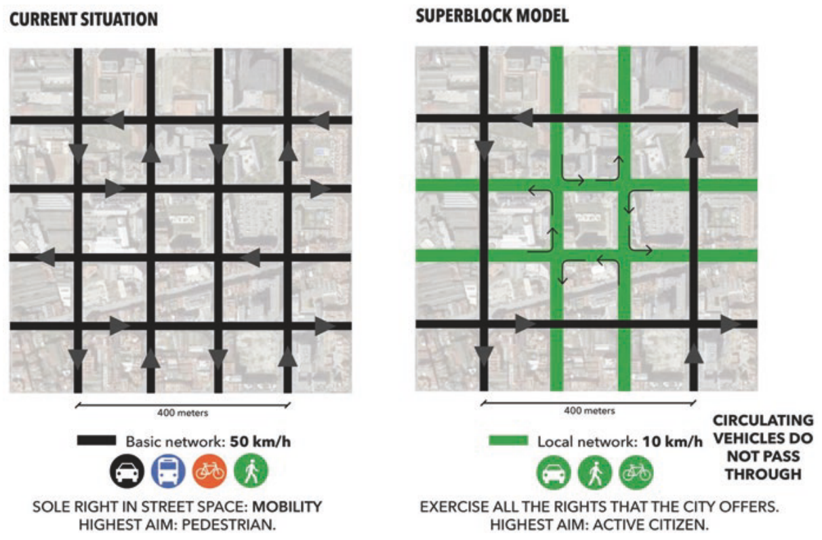
\includegraphics[scale=0.5]{bcn_superblocks_rueda_2018.png}
\caption{Barcelona Superblocks schema (Rueda, 2018).}
\label{fig:Barcelona Superblocks schema}
\end{figure}

\subsection {The Braess Paradox}

Among one of the most interesting and intriguing effects that defies the common understanding for operating in the urban infrastructures is the so-called Braess Paradox. It explains the counter-intuitive observation that adding more links to a given network, such as a transportation one, can slow down overall traffic flow. It is caused by the selfishly behavior of the entities that are moving in the network when trying to optimize individually their travel time (or cost). It causes to get away from the system optimum. that contrary to the real behavior, requires some level of collaboration between the agents \citep{Braess1969}.

\section {Research questions}

\begin{itemize}
    \item Are there too many streets for cars that actually are causing bigger congestion?
    \item If adding new roadways links leads to increased congestion, according to Braess, may removing streets for vehicles cause improvement of traffic, as expected by the Superblocks plan?
    \item Can we apply the counter-intuitive Braess’ Paradox effects for our own benefit in the planning of cities?
\end{itemize}

\section{Individual contributions}

\section{Introduction and Motivations}

\section{Description of the Model}

\section{Implementation}

\section{Simulation Results and Discussion}

\section{Summary and Outlook}

\section{References}






\end{document}  



 
